% fig_ibr_rxplane.tex
% TR-29: R-X plane showing three Mho zones and IBR fault impedance locus
%
% Mho circle geometry (Z_reach = jX_R, purely reactive line):
%   Centre = (0, X_R/2),  Radius = X_R/2
%   Circle passes through origin.
%
% Zone parameters (TR-18 settings):
%   Zone 1: X_R = 0.040 pu  -> centre (0, 0.020),  radius 0.020
%   Zone 2: X_R = 0.060 pu  -> centre (0, 0.030),  radius 0.030
%   Zone 3: X_R = 0.090 pu  -> centre (0, 0.045),  radius 0.045
%
% Line impedance locus: Z_line = j*0.05*alpha, alpha in [0,1]
%   This is a segment on the +jX axis from 0 to j0.050
%
% Key fault points:
%   alpha=0.50: Z_m = j0.025  (inside Z1, inside Z2)
%   alpha=0.80: Z_m = j0.040  (at Z1 boundary)
%   alpha=0.82: Z_m = j0.041  (just outside Z1, inside Z2)
%   alpha=1.00: Z_m = j0.050  (end of line, inside Z2, outside Z1)
%
% IBR key finding: Z_m = alpha * Z_line (identical to SG)
%   BUT: V_relay = k_ibr * alpha * Z_line <= 0.010 pu (always < V_min_self=0.10)
%   AND: for k_ibr < 0.10: relay blocked by I_min threshold

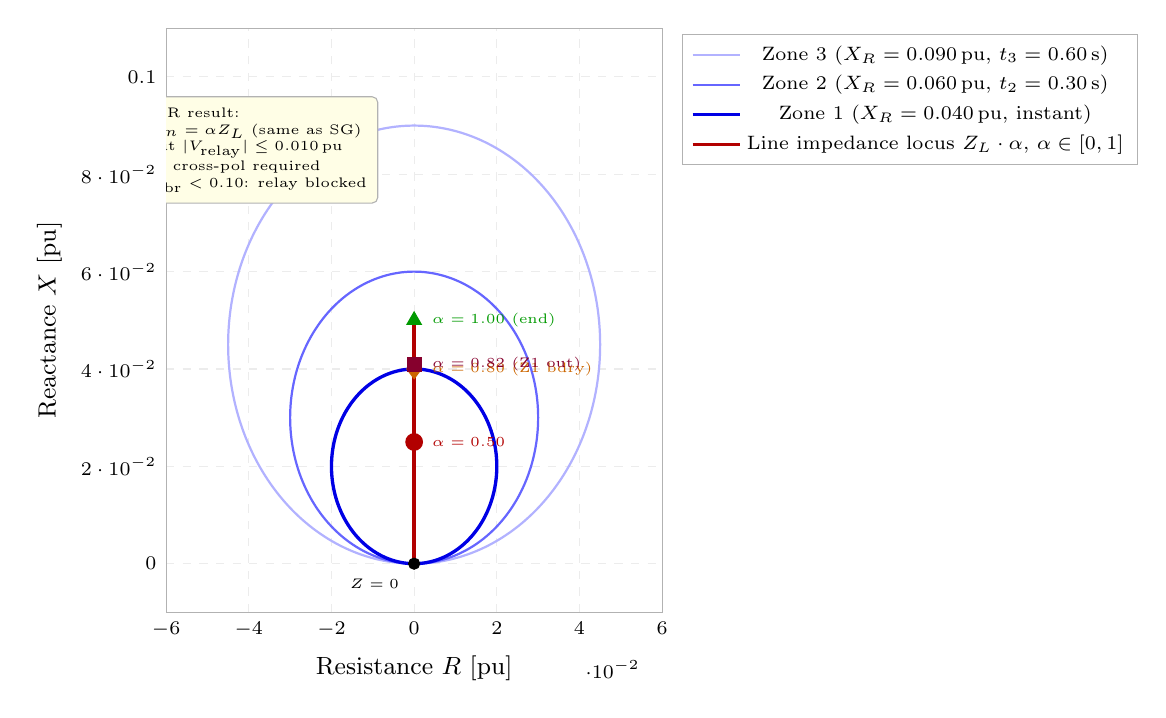
\begin{tikzpicture}
\begin{axis}[
  name         = rxax,
  width        = 0.65\textwidth,
  height       = 9.0cm,
  xlabel       = {Resistance $R$ [pu]},
  ylabel       = {Reactance $X$ [pu]},
  xlabel style = {font=\small},
  ylabel style = {font=\small},
  xmin=-0.06, xmax=0.06,
  ymin=-0.010, ymax=0.110,
  xtick        = {-0.06,-0.04,-0.02,0,0.02,0.04,0.06},
  xticklabel style={font=\scriptsize},
  ytick        = {0, 0.02, 0.04, 0.06, 0.08, 0.10},
  yticklabel style={font=\scriptsize},
  grid         = major,
  grid style   = {gray!15, dashed},
  tick style   = {draw=none},
  axis line style={gray!60},
  legend style={at={(1.04,0.99)}, anchor=north west, font=\scriptsize,
                draw=gray!60},
]

% ---- Mho circles  (parametric: x=r*cos(t), y=cy+r*sin(t)) ----
% Zone 3 (outermost) drawn first so inner zones overlap
\addplot[blue!30, thick, domain=0:360, samples=200, smooth]
  ({0.045*cos(x)}, {0.045 + 0.045*sin(x)});
\addlegendentry{Zone 3 ($X_R=0.090$\,pu, $t_3=0.60$\,s)}

\addplot[blue!60, thick, domain=0:360, samples=200, smooth]
  ({0.030*cos(x)}, {0.030 + 0.030*sin(x)});
\addlegendentry{Zone 2 ($X_R=0.060$\,pu, $t_2=0.30$\,s)}

\addplot[blue!90!black, very thick, domain=0:360, samples=200, smooth]
  ({0.020*cos(x)}, {0.020 + 0.020*sin(x)});
\addlegendentry{Zone 1 ($X_R=0.040$\,pu, instant)}

% ---- Line impedance locus ----
\addplot[red!70!black, very thick, mark=none]
  coordinates {(0,0) (0,0.050)};
\addlegendentry{Line impedance locus $Z_L\cdot\alpha$, $\alpha\in[0,1]$}

% ---- Key fault points ----
% alpha=0.50: Z_m = j0.025 (inside Z1)
\addplot[mark=*, mark size=3pt, red!70!black, only marks]
  coordinates {(0, 0.025)};
\node[right=3pt, font=\tiny, red!70!black] at (axis cs:0, 0.025)
  {$\alpha=0.50$};

% alpha=0.80: Z_m = j0.040 (Zone 1 boundary)
\addplot[mark=diamond*, mark size=3.5pt, orange!80!black, only marks]
  coordinates {(0, 0.040)};
\node[right=3pt, font=\tiny, orange!80!black] at (axis cs:0, 0.040)
  {$\alpha=0.80$ (Z1 bdry)};

% alpha=0.82: Z_m = j0.041 (just outside Z1)
\addplot[mark=square*, mark size=2.5pt, purple!70!black, only marks]
  coordinates {(0, 0.041)};
\node[right=3pt, font=\tiny, purple!70!black] at (axis cs:0, 0.041)
  {$\alpha=0.82$ (Z1 out)};

% alpha=1.00: Z_m = j0.050 (end of line)
\addplot[mark=triangle*, mark size=3pt, green!60!black, only marks]
  coordinates {(0, 0.050)};
\node[right=3pt, font=\tiny, green!60!black] at (axis cs:0, 0.050)
  {$\alpha=1.00$ (end)};

% ---- Origin ----
\addplot[mark=*, mark size=2pt, black, only marks]
  coordinates {(0,0)};
\node[below left=2pt, font=\tiny] at (axis cs:0,0) {$Z=0$};

% ---- Annotation box ----
\node[draw=gray!60, fill=yellow!10, rounded corners=2pt,
      font=\tiny, align=left, inner sep=4pt]
  at (axis cs:-0.038, 0.085)
  {IBR result:\\
   $Z_m = \alpha Z_L$ (same as SG)\\
   but $|V_{\rm relay}| \leq 0.010$\,pu\\
   $\Rightarrow$ cross-pol required\\
   $k_{\rm ibr}<0.10$: relay blocked};

\end{axis}
\end{tikzpicture}
